% $Id: AllegProposal.tex,v 1.8 2000/07/05 21:02:12 culver Exp $
% AllegProposal.tex
% by A. Thall
% 13. Feb 2003
%
% Small edits and a few additions made by R. Roos
% 21 Jan 2007
% Most particularly, the "box" around the thesis statement has been removed,
% section titles have been modified. The section named "Prior work II" has
% been commented out. The \topmargin has been changed to -.5in and the
% change to \parindent has been commented out.
% The filename "nausicaa.eps" has been changed to simply "nausicaa" so that
% pdflatex can be used on the file (and a file named "nausicaa.pdf" has
% been created using the "epstopdf" command).
% Several subsections have been added to illustrate subsection usage.
% The word "comp" has been replaced by "project" or "thesis" throughout.
% Other small changes have been made.
%
% This document provides a sample Senior Project Proposal template for use
% by students in Allegheny's CS and Applied Computing programs.

\NeedsTeXFormat{LaTeX2e}
\documentclass[11pt]{article}
\usepackage[utf8]{inputenc}
%The following is used by WinEdt to set up cross-referencing to the BibTeX files
%It is NOT commented out---the comment lets it be simply ignored by non-WinEdt LaTeX compilers

%GATHER{mybibtexDB.bib}

\usepackage{setspace}
\usepackage{amsmath}
\usepackage{amssymb}
\usepackage{epsfig}
\usepackage{fancybox}
\usepackage{listings}
\usepackage{algo}
\usepackage{url}
\usepackage{graphicx}
\usepackage{subcaption}

\setlength{\textheight}{9in}
\setlength{\textwidth}{6in}
\setlength{\oddsidemargin}{.25in}
\setlength{\topmargin}{-.5in}  % changed from -.25 by RSR on 1/21/07
%\parindent .5in    % commented out by RSR 1/21/07

%put words in the hyphenation statement if you want to enforce
%how LaTeX should break them (or not) at the end of a line.
%\hyphenation{repre-sen-tations problems exact linear}
\hyphenation{itself}

%%%%%
%% Commented out -- RSR, 1/21/07
%%%%%
% The following provides a box to surround the thesis statement
%\newenvironment{Thesis}%
%{\begin{Sbox}\begin{minipage}{.95\linewidth}}%
%{\end{minipage}\end{Sbox}\begin{center}\fbox{\TheSbox}\end{center}}

\title{Relatório Parcial: Ano 2}
\author{Isaac L.\ Santos\ Sacramento \\ Orientador: Mauro Roisenberg}

\begin{document}

% You can specify a language and other options for
% the code-formatting "listings" package
\lstset{language=C++,basicstyle=\small,
        stringstyle=\ttfamily,showstringspaces=false}

\singlespace
\maketitle

\begin{abstract}                % ~350 words max
Neste relatório são apresentadas as atividades realizadas no
período de outubro de 2016 até abril de 2017. Neste período foram realizados estudos e experimentos relacionados à aplicação
de \textit{Redes Neurais Convolucionais} para realizar predição de propriedades geofísicas e hiper-resolução de imagens pós-inversão.
Estas atividades estão descritas nas seções a seguir.

\end{abstract}

\doublespace
% This sets section-numbering to only include Section and Subsection numbers
\setcounter{secnumdepth}{2}

\section{Introdução}

No período de outubro de 2016 até abril de 2017 foram exploradas as frentes de trabalho relacionadas ao uso
das redes neurais convolucionais no processo de simulação geoestatística e na super-resolução de propriedades pós-inversão.
Após o estudo dos métodos de simulação multiponto, foram realizados experimentos com o intuito de obter um modelo de rede neural convolucional
capaz de aprender os padrões das imagens de treinamento e reproduzi-los posteriormente na geração de novas realizações estatisticamente compatíveis.
Nesta etapa, os experimentos foram implementados em linguagem \textit{MATLAB} e com auxílio da biblioteca de aprendizagem de máquina (\textit{Machine Learning}),
\textit{TensorFlow}. Esta biblioteca permite a implementação de modelos de redes neurais convolucionais em linguagem Python. 
A primeira parte dos experimentos consistiu em estudar um modelo de rede neural convolucional
capaz de realizar a predição de uma função matemática não-linear. Com este experimento se deseja
obter um modelo que possa ser estendido para realizar predição de propriedades petrofísicas e que,
posteriormente, estas predições possam ser combinadas de modo a realizar simulações
geoestatísticas multiponto a partir de uma dada imagem de treinamento.

O processo de inversão sísmica disponibiliza artefatos cujos valores oscilam em torno
do valor valor médio da propriedade invertida (\textit{maximum-a-posteriori}). Com isso,
o resultado de inversão é capaz de evidenciar regiões de reservatório, entretanto,
as imagens possuem baixa e média resolução. Mais precisamente, as imagens são limitadas
pela banda de frequência da sísmica e da \textit{wavelet} utilizada no processo de inversão, além de um modelo
de baixa frequência incorporado ao modelo de inversão.
Assim, a segunda parte dos experimentos, consistiu em experimentar as redes neurais convolucionais
para incorporar maior resolução às imagens de impedância acústica obtidas com o processo
de inversão sísmica. 

\section{Redes Neurais Convolucionais}

As redes convolucionais, também chamadas de redes neurais convolucionais (CNN),
são um tipo de rede neural especializada em processamento de dados que possuam uma
topologia conhecida e em forma de grade. Exemplos deste tipo de dado são as séries
temporais, que podem ser vistas como uma grade em uma dimensão (1D) com amostras
em intervalos de tempo regulares, e dados de imagem, que podem ser pensados como
uma grade 2D de \textit{pixels}. As redes convolucionais são um tipo de rede neural
que usa a operação de convolução no lugar de multiplicação de matrizes em pelo menos uma
de suas camadas. A operação de convolução costuma ser denotada com um asterisco (Eq. \ref{eq:1}).
Na Equação. \ref{eq:1}, $x$ refere-se ao conjunto de imagens de entrada, uma sequência multidimensional
de dados, e $w$ é denominado \textit{kernel} ou filtros, uma sequência multidimensional de parâmetros otimizados pelo algoritmo
de aprendizagem.
\begin{equation}
 s(t) = (x * w)(t)
 \label{eq:1}
\end{equation}

\subsection{Predição da Função Seno}
O uso do seno como experimento inicial buscou alcançar um modelo de
rede neural convolucional capaz de realizar a aproximação desta função utilizando
imagens da própria função seno como entrada para o treinamento.
A função seno foi arbitrariamente escolhida para
representar um conjunto de treinamento não-linear, mas simples o
suficiente, que permitisse obter um modelo de previsão,
ao invés de classificação. É importante ressaltar que este modelo deve ser
aprimorado e adaptado para a resolução de problemas com conjuntos de dados
do mundo real.

O conjunto de entrada das redes neurais convolucionais
são imagens de treinamento, a partir das quais se deseja extrair padrões espaciais
que permitam realizar previsão. Para construir o conjunto de entradas da rede,
foi gerada uma matriz, na qual cada linha representa uma imagem em 1D
composta por $10$ valores subsequentes da função seno, o valor seguinte é o que se
deseja prever. Desta forma, o experimento se assemelha à predição de uma série temporal.
Deve ficar claro, porém, que os valores dos ângulos de entrada para a função
seno não são utilizados como entrada da rede convolucional, de modo que a predição
deverá ocorrer baseada no aprendizado do padrão da curva existente no conjunto de
de $10$ valores da função. Todo o conjunto é inicialmente composto por $90$ imagens.

O modelo foi implementado de forma incremental, em busca do melhor ajuste dos
seus hiper-parâmetros. Foi realizado um estudo de sensibilidade dos hiper-parâmetros do
modelo convolucional para obter uma configuração capaz de realizar
a previsão da função seno. A seguir, são listados os parâmetros estudados,
os quais foram testados para diferentes valores e combinações entre eles.
 \begin{description}
   \item[taxa de aprendizagem] taxa de aprendizado utilizada pelo algoritmo de treinamento Gradiente Descendente.
   \item[tamanho do batch] número de imagens utilizadas em cada iteração do treinamento.
   \item[número de \textit{kernels}] número de matrizes de pesos convolvidas com as imagens de entrada em cada camada convolucional.
   \item[dimensão dos \textit{kernels}] dimensão dos \textit{kernels} utilizados na convolução.
 \end{description}

De acordo com os testes realizados, o tamanho do \textit{batch},
do conjunto de entrada da rede, e a taxa de aprendizado foram
os parâmetros que causaram maior oscilação no comportamento da
rede durante o aprendizado. O estudo de sensibilidade dos hiper-parâmetros
foi combinado com a definição do modelo convolucional propriamente dito.
Neste sentido, inicialmente foi definido um modelo arbitrário composto por uma camada convolucional,
uma camada de \textit{pooling} e uma camada completamente conectada (\textit{Fully Connected}),
na qual todos os pesos e \textit{biases} na saída da camada de \textit{pooling} são conectados a um único
neurônio na camada de saída. Posteriormente, este modelo foi estendido para duas camadas
convolucionais intercaladas por duas camadas de \textit{pooling}, ilustrado na Figura \ref{fig:model}. Intuitivamente,
em razão da não linearidade da função seno, na saída da camada
convolucional foram testadas funções de ativação não-lineares.
Entretanto, esta configuração atribuiu um comportamento instável ao modelo, não convergente.
Por outro lado, ao abandonar o uso das funções de ativação não-lineares, a rede apresentou convergência no processo de treinamento,
entretanto para intervalos menores e contidos no intervalo de predição esperado, de $[-1,1]$.

\begin{figure}[htp]
\begin{center}
  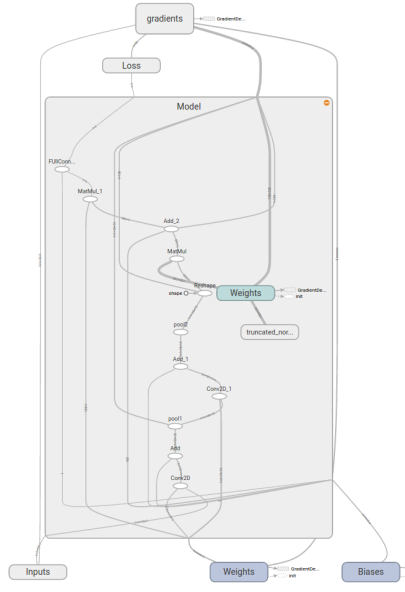
\includegraphics[width=0.5\textwidth]{fig/modelo}
  \caption{Modelo básico para previsão da função seno.}
  \label{fig:model}
\end{center}
\end{figure}

Os resultados dos experimentos evidenciaram o potencial de pesquisa em relação
ao desenvolvimento de um modelo de rede neural convolucional capaz de realizar
predição de propriedades petrofísicas baseado no uso de imagens já conhecidas da
mesma propriedade. Este método se assemelha ao processo de simulação geoestatística
multiponto, já discutido em relatórios passados.

\section{Super-resolução em Imagens Pós-inversão Sísmica}
A super-resolução tem um papel importante na visão computacional \cite{DongLoy2016}.
Métodos baseados em interpolação são fáceis de implementar e amplamente utilizados,
entretanto estes métodos sofrem de falta de expressividade, uma vez que modelos lineares
não são capazes de expressar dependências complexas entre as entradas e as saídas \cite{HsiehAndrews1978}.
Na prática tais métodos falham na tentativa de prever adequadamente detalhes de alta frequência
levando a saídas de alta resolução borradas. Efeito semelhante ocorre durante a inversão sísmica,
na qual as imagens resultantes apresentam resolução limitada e contornos borrados. Assim, um modelo
de rede convolucional foi testado para atribuir às imagens de inversão sísmica para impedância
elementos de alta frequência.

O modelo de rede adotado neste experimento foi adaptado para o domínio da geoestatística. Os testes
foram realizados com pares de imagens de impedância acústica esparsa (maior resolução) e 
imagens dos valores de \textit{maximum-a-posteriori} (MAP)(baixa resolução) da impedância acústica,
ambas obtidas pelo processo de inversão sísmica. Os testes realizados compreenderam as seguintes etapas:
 \begin{itemize}
   \item Conversão para escala de cinza
   \item Treinamento da rede
   \item Normalização das imagens
   \item Cálculo do grau de similaridade das imagens
   \item Recuperação dos valores de impedância
 \end{itemize}

As redes neurais convolucionais aplicadas à super-resolução funcionam por meio da classificação de cada pixel da 
imagem de treinamento dentro de uma determinada faixa de valores inteiros. Por conta desta
característica, as imagens de impedância MAP (baixa resolução)
e esparsa (alta resolução), foram convertidas para tons de cinza no intervalo de
0 e 255. O treinamento da rede foi realizado com o uso de pares de imagens equivalentes (baixa e alta resolução)
como entrada e alvo, respectivamente, para o modelo, de modo que o aprendizado ocorre ao tentar aproximar a
imagem de baixa resolução para a de alta resolução. Após o treinamento um conjunto de imagens de baixa resolução
foi  selecionado para teste, as imagens obtidas na saída da rede foram normalizadas para o intervalo de 0 a 1
para o cálculo do seu grau de similaridade com as imagens de alta resolução desejadas.
A Transformada Rápida de Fourier (FFT) foi utilizada como método de comparação entre as imagens calculadas pela rede
e as imagens de alta resolução de impedância esparsa. A métrica de similaridade entre as imagens é calculada usando a fórmula \ref{eq:2}, baseada
no espectro de frequência das imagens.

\begin{equation}
 C = \frac{ (\sum_{i=1}^{N}{F_{1i}F_{2i}} - N \bar{F}_1\bar{F}_2 )^2 }{ (\sum_{i=1}^{N}{|F_{1i}|^2} - N{\bar{F}^2}_1)( \sum_{i=1}^{N}{|F_{2i}|^2} - N{\bar{F}^2}_2 ) }
 \label{eq:2}
\end{equation}

Para cada frequência, um valor de intensidade é obtido das partes real e complexa da Transformada de Fourier.
Por conta da limitação de memória para processamento, foram utilizadas sub-imagens (32\textit{px} x 32\textit{px}) das
imagens de impedância. $F_{1i}$ é o valor de intensidade do i-ésimo pixel da primeira imagem, enquanto $F_{2i}$
é o valor de intensidade do i-ésimo pixel da segunda imagem. $\bar{F}_1$ e $\bar{F}_2$ representam os valores
de frequência média de cada imagem. A métrica varia no intervalo de 0 a 1, sendo que, similaridade igual a 1
representa a comparação entre imagens iguais.

A métrica $C$ foi calculada entre as imagens obtidas pela rede e as imagens de alta resolução de impedância esparsa, também, entre estas e
as imagens de MAP de impedância (baixa resolução). Com a utilização da métrica $C$, ficou evidente que as imagens em alta resolução obtidas com a rede apresentaram
maior similaridade com a imagem de impedância esparsa (alta resolução) e que, de fato a rede foi capaz de agregar elementos de
alta frequência à maioria das imagens de baixa resolução (MAP de impedância), em torno de $84\%$. As Figuras (\ref{fig:sfig1},\ref{fig:sfig2},\ref{fig:sfig3} e \ref{fig:sfig4})
apresentam resultados obtido pela rede e os respectivos valores do índice de similaridade entre as imagens.
\begin{figure}[htp]
\begin{subfigure}{.5\textwidth}
  \centering
  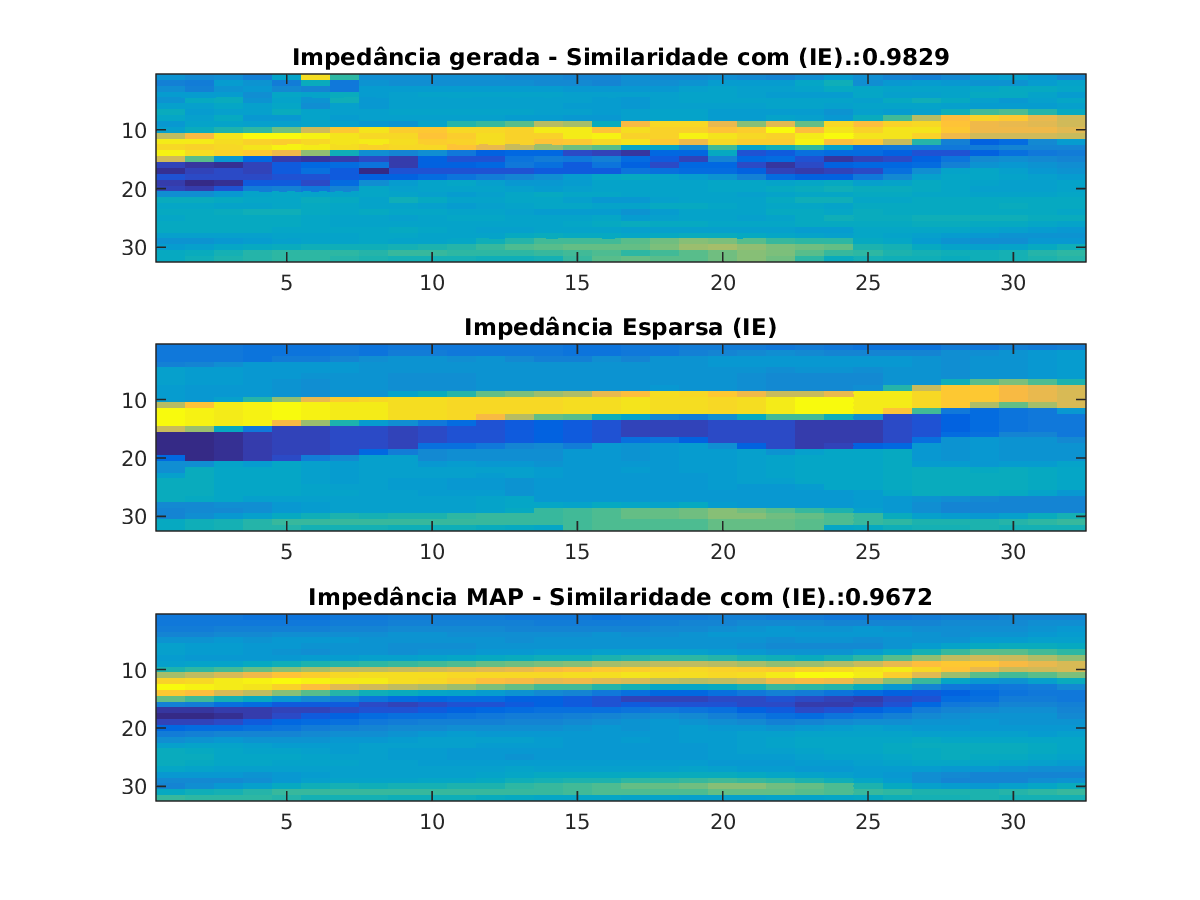
\includegraphics[width=.9\linewidth]{fig/7}
  \caption{}
  \label{fig:sfig1}
\end{subfigure}%
\begin{subfigure}{.5\textwidth}
  \centering
  
\includegraphics[width=.9\linewidth]{fig/5}
  \caption{}
  \label{fig:sfig2}
\end{subfigure}
\begin{subfigure}{.5\textwidth}
  \centering
  
\includegraphics[width=.9\linewidth]{fig/19}
  \caption{}
  \label{fig:sfig3}
\end{subfigure}
\begin{subfigure}{.5\textwidth}
  \centering
  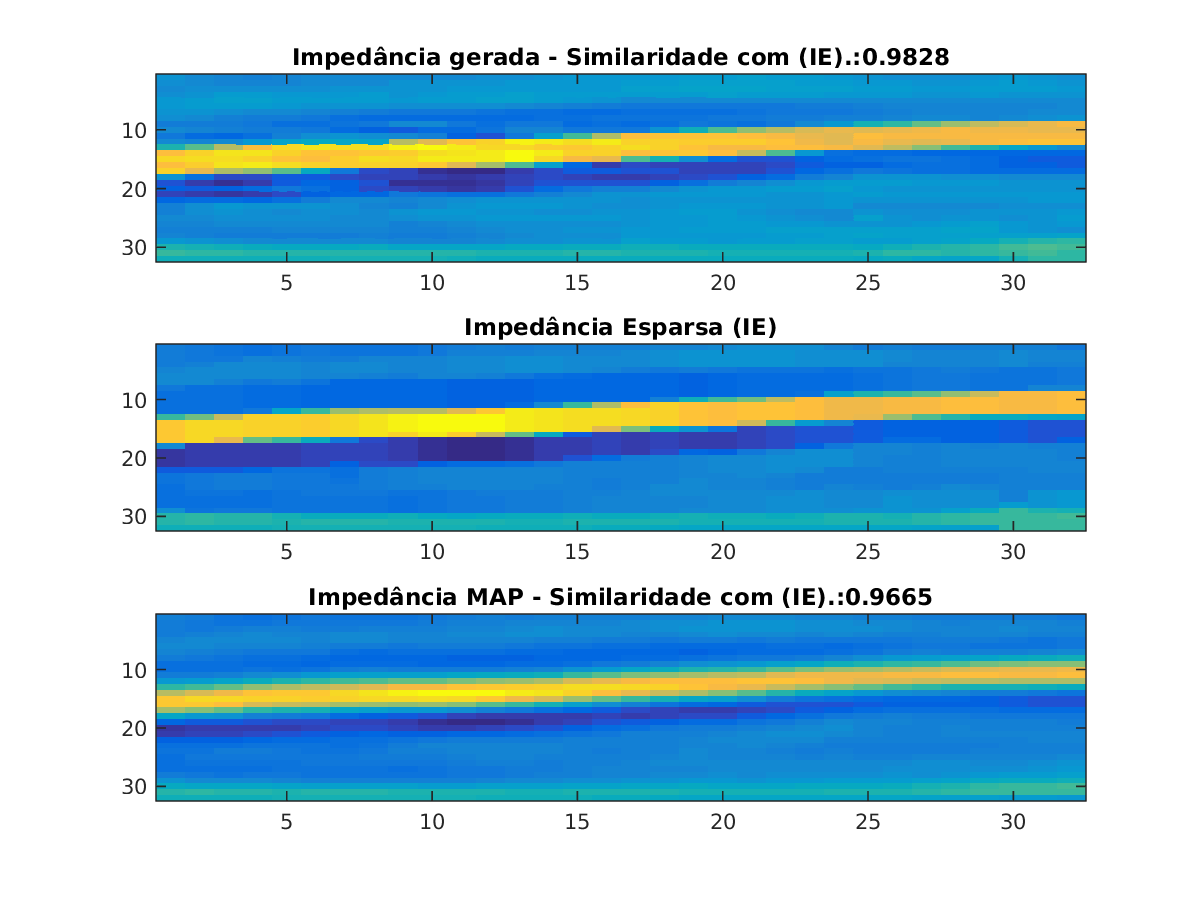
\includegraphics[width=.9\linewidth]{fig/25}
  \caption{}
  \label{fig:sfig4}
\end{subfigure}
 \caption{Amostras de impedâncias obtidas pela CNN (alta resolução), esparsas (alta resolução) e MAP (baixa resolução).}
 \label{fig:sf}
\end{figure}

\section{Conclusões}
Os experimentos apresentados neste relatório compreenderam o uso das redes neurais convolucionais para previsão da função seno a partir de
imagens da própria função. Estes experimentos se mostraram promissores, pois as redes apresentaram evolução no treinamento e se tornaram mais estáveis quanto
à previsão de valores reais. O modelo estudado deve ser aprimorado para alcançar as predições mais próximas aos limites de intervalo da função.
As redes convolucionais se mostraram ainda mais promissoras quando utilizadas para o aumento de resolução de imagens
de impedância acústica obtidas pelo processo de inversão sísmica.
As etapas seguintes referentes a este experimento consistem em definir um fluxograma de atividades para hiper-resolução das imagens de inversão, a implementação para
tornar a rede capaz de aprender imagens maiores, a implementação
do modelo de super-resolução atual para amostragem em \textit{batch}, ao invés de pixel a pixel, e a investigação
de um modelo de rede convolucional classificadora capaz de resolver o problema de simulação multiponto baseada em imagem de treinamento.

\nocite{*}

\begin{spacing}{1}
   \bibliographystyle{plain}
   \bibliography{mybibtexDB}
 \end{spacing}

\end{document}
\grid
